%-----------------------------------------------------------------------------
%
%               Template for sigplanconf LaTeX Class
%
% Name:         sigplanconf-template.tex
%
% Purpose:      A template for sigplanconf.cls, which is a LaTeX 2e class
%               file for SIGPLAN conference proceedings.
%
% Guide:        Refer to "Author's Guide to the ACM SIGPLAN Class,"
%               sigplanconf-guide.pdf
%
% Author:       Paul C. Anagnostopoulos
%               Windfall Software
%               978 371-2316
%               paul@windfall.com
%
% Created:      15 February 2005
%
%-----------------------------------------------------------------------------


\documentclass{sigplanconf}

% The following \documentclass options may be useful:

% preprint      Remove this option only once the paper is in final form.
% 10pt          To set in 10-point type instead of 9-point.
% 11pt          To set in 11-point type instead of 9-point.
% authoryear    To obtain author/year citation style instead of numeric.

\usepackage{amsmath}
\usepackage{graphicx}


\begin{document}

\special{papersize=8.5in,11in}
\setlength{\pdfpageheight}{\paperheight}
\setlength{\pdfpagewidth}{\paperwidth}

\conferenceinfo{CONF 'yy}{Month d--d, 20yy, City, ST, Country} 
\copyrightyear{20yy} 
\copyrightdata{978-1-nnnn-nnnn-n/yy/mm} 
\doi{nnnnnnn.nnnnnnn}

% Uncomment one of the following two, if you are not going for the 
% traditional copyright transfer agreement.

%\exclusivelicense                % ACM gets exclusive license to publish, 
                                  % you retain copyright

%\permissiontopublish             % ACM gets nonexclusive license to publish
                                  % (paid open-access papers, 
                                  % short abstracts)

\titlebanner{banner above paper title}        % These are ignored unless
\preprintfooter{short description of paper}   % 'preprint' option specified.

\title{Kernel Fusion: from Halide to OpenCL}

\authorinfo{Hsin-Liang Yeh}
           {Dept. of Computer Science and Information Engineering
           
           National Taiwan University}
           {sting47@gmail.com}
\authorinfo{Name2\and Name3}
           {Affiliation2/3}
           {Email2/3}

\maketitle

\begin{abstract}
\quad\ \ In image processing area, there are many algorithms that will need to execute their algorithm multiple times to one image. To this kind of algorithms, there will be redundant overheads between kernels. We can apply kernel fusion to eliminate these overheads. 
    
    Halide now provides a way to do kernel fusion, but using this way will cause redundant works and redundant pixels accessed. We introduce another way to perform kernel fusion without redundant works in order for Halide to add this way to OpenCL CodeGen and improve the performance of kernel fusion.
\end{abstract}

\category{CR-number}{subcategory}{third-level}

% general terms are not compulsory anymore, 
% you may leave them out
\terms
term1, term2

\keywords
keyword1, keyword2

\section{Introduction}
\quad\ \ In image processing area, it’s common to use multiple filters on one image. So we tried to optimize this kind of image processing.

    Focus on examples that uses more than one filter, we choose the blur algorithm and blur one image many times for a basic example. If we are blurring one image many times, we will first create a blur kernel by using clCreateKernel. And then enqueue this kernel many times by using clEnqueueNDRangeKernel.
    
    But every time we enqueue the kernel, we need to return back to the host (normally the CPUs) from the devices (usually the CPUs or GPUs) and do some setup for the next kernel being enqueued, including redirect the previous kernel’s output into the next  kernel’s input arguments by resetting them using clSetKernelArg. These movements can be treated as overhead and can cause performance reduction if many kernels are enqueued.
    
	So we tried to reduce or eliminate these overhead by the concept, kernel fusion. This means to fuse several kernel into one kernel, so we don’t need to do the setup for multiple kernels.
	
	In order to do kernel fusion, there is a main constraint, how to sync the data. In the original way, the next kernel will be enqueued after the previous kernel finished, which means all the work group finish the previous kernel. So the input of the next kernel will be guaranteed correctness. But in kernel fusion, the correctness of the data can’t be guaranteed because we fuse several kernels into one kernel.
	
	Since for stencil algorithms, we need the pixels around the target pixel to calculate the target pixel’s result. But when we fuse several kernels into one, the next kernel can not obtain the result from the previous kernel and causing correctness violation.

\section{Background}
\subsection{Halide}
\quad\ \ Halide\cite{halideori} is a new programming language designed to make it easier to write high-performance image processing code on modern machines. Its current front end is embedded in C++. Compiler targets include x86/SSE, ARM v7/NEON, CUDA, Native Client, and OpenCL.

    Halide represents a systematic model of the tradeoff space fundamental to stencil pipelines, a schedule representation which describes concrete points in this space for each stage in an image processing pipeline, and an optimizing compiler for the Halide image processing language that synthesizes high performance implementations from a Halide algorithm and a schedule. Combining this compiler with stochastic search over the space of schedules enables terse, composable programs to achieve state-of-the-art performance on a wide range of real image processing pipelines, and across different hardware architectures, including multicores with SIMD, and heterogeneous CPU and GPU execution.

\subsection{OpenCL}
\quad\ \ OpenCL (Open Computing Language) is an open royalty-free standard for general purpose parallel programming across CPUs, GPUs and other processors, giving software developers portable and efficient access to the power of these heterogeneous processing platforms.

    OpenCL supports a wide range of applications, ranging from embedded and consumer software to HPC solutions, through a low-level, high-performance, portable abstraction. By creating an efficient, close-to-the-metal programming interface, OpenCL will form the foundation layer of a parallel computing ecosystem of platform-independent tools, middleware and applications. OpenCL is particularly suited to play an increasingly significant role in emerging interactive graphics applications that combine general parallel compute algorithms with graphics rendering pipelines.
    
    OpenCL consists of an API for coordinating parallel computation across heterogeneous processors; and a cross-platform programming language with a well- specified computation environment. The OpenCL standard: Supports both data- and task-based parallel programming models, Utilizes a subset of ISO C99 with extensions for parallelism, Defines consistent numerical requirements based on IEEE 754, Defines a configuration profile for handheld and embedded devices, Efficiently interoperates with OpenGL, OpenGL ES and other graphics APIs.

\section{Methodology}
\subsection{Fix correctness violation}
\quad\ \ There are two ways to fix the correctness violation mentioned at the last paragraph in the previous chapter. Seeing Figure
~\ref{fig:my_label1}, one is to add barrier between kernels so the next kernel will not start until all work group finish the previous kernel and stored the result into global memory. The other one is to do redundant works, calculating all the data needed itself in every work group.

\begin{figure}[hbtp]
\centering
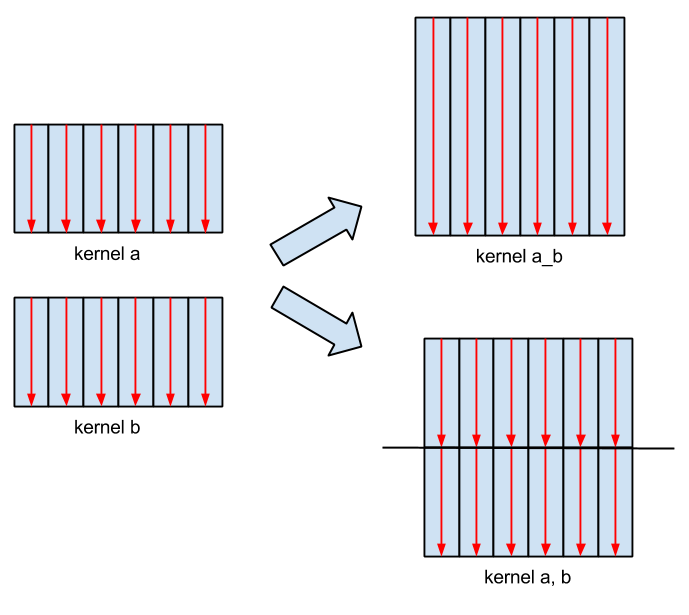
\includegraphics[width=7cm]{img/kernel-fusion.png}
\caption{kernel fusion}
\label{fig:my_label1}
\end{figure}

\subsection{Halide schedule compute\_at}
\quad\ \ Halide provide a schedule named “compute\_at”, and it can fuse multiple kernels into one kernel. The schedule uses the second way, doing redundant works to calculate the data needed itself. The main disadvantage of this way is, the more the kernels fused, the more the redundant works shows.

	For example, Figure~\ref{fig:my_label2} shows the pixels accessed to calculate one pixel’s result. The pink part represents the pixels accessed in the kernel.The algorithm is to obtain the pixel on the target pixel’s left and right, and calculate the sum of the two pixels and the target pixel. The example shows processing the image using the algorithm two times. We can see every kernel access two extra pixels except the target pixel.
	
\begin{figure}[hbtp]
\centering
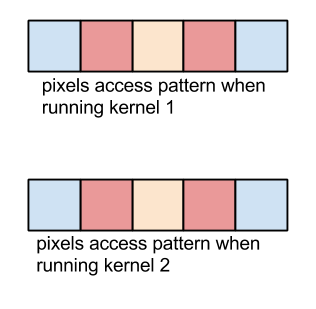
\includegraphics[width=6cm]{img/figure2.png}
\caption{accessing pattern of 2 kernels}
\label{fig:my_label2}
\end{figure}

    Figure~\ref{fig:my_label3} shows the calculating flow of doing one dimension blur algorithm twice, and applying kernel fusion by doing redundant works. We can see the number of pixels accessed are five in the first kernel, and three in the second kernel.
	
\begin{figure}[hbtp]
\centering
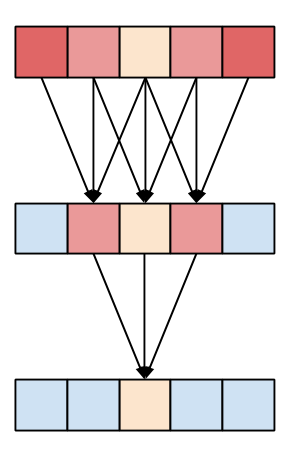
\includegraphics[width=5cm]{img/figure3-6(for-paper).png}
\caption{Example of the calculating flow when doing redundant works}
\label{fig:my_label3}
\end{figure}
	
	Figure~\ref{fig:my_label4} shows the pixels accessed to calculate one pixel’s result if we use Halide schedule, compute\_at. The pink part represents pixels accessed in the first kernel. The burgundy part represents the extra pixels accessed in the second kernel. We can see if we want to eliminate the dependency without barrier, we need to access two extra pixels than original.
	
\begin{figure}[hbtp]
\centering
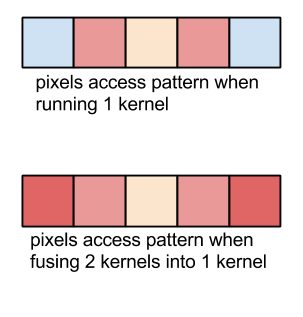
\includegraphics[width=6cm]{img/figure3.png}
\caption{accessing pattern of compute\_at}
\label{fig:my_label4}
\end{figure}
	
	Figure~\ref{fig:my_label5} shows the accessing pattern using kernel fusion when processing an image with a blur algorithm accessing the 8 pixels around the target pixel. The pink part represents pixels accessed in the first kernel. The burgundy part represents the extra pixels accessed in the second kernel. We can see when blurring the image 2 times, the increasing redundant works are to calculate 16 pixels compared to the original version. And the redundant works will be calculating 24 pixels compared to only fuse 2 kernels into one if we fuse 3 kernels into one kernel. So the redundant works grow fast according to how many kernels we fuse.

\begin{figure}[hbtp]
\centering
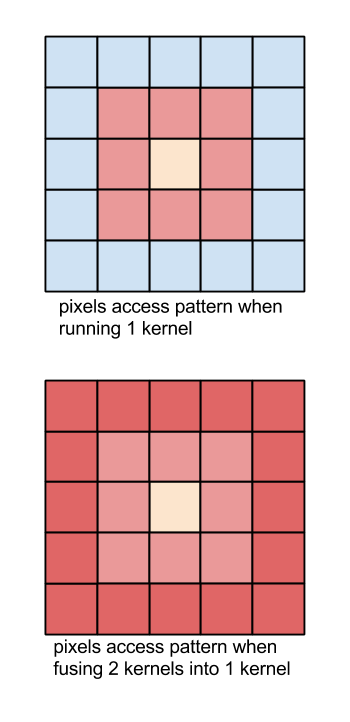
\includegraphics[width=5cm]{img/figure4.png}
\caption{accessing pattern of compute\_at 2}
\label{fig:my_label5}
\end{figure}

\subsection{Approach: enqueue\_kernel}
\quad\ \ We implement our enqueue\_kernel feature on an Open-Source Project - POCL\cite{poclori} (Portable Computing Language.) It is an OpenCL implementation. Our approach will help the user to branch to the new kernel at runtime by using the “block” which is defined by the Clang\cite{clangori} (a compiler front end for the C, C++, Objective-C and Objective-C++ programming languages) and it can be used like a function pointer. According to the OpenCL 2.0 spec\cite{opencl2.0spec}, enqueue\_kernel’s second input argument is “kernel\_enqueue\_flags\_t flags”. The flags can be CLK\_ENQUEUE\_FLAGS\_NO\_WAIT, CLK-
\_ENQUEUE\_FLAGS\_WAIT\_KERNEL and CLK\_ENQUEUE\_FLA-
GS\_WAIT\_WORK\_GROUP.

    Figure~\ref{fig:my_label6} is a flowchart presenting our approach. We implement our approach pre-parser inside the host OpenCL API clCreateProgramWithSource. When the kernel source code are input, our pre-parser will process the source code according to which flag is specified.

	Our approach can perform full functionality of the last flag mentioned, but leave the first and the second flag limited functionality. We add a pre-parser before compiling the kernel source code to binary program (before clCreateProgramWithSource.) to do setup for the enqueue\_kernel function according to the kernel\_enqueue\_flags\_t. 
	
\begin{figure}[hbtp]
\centering
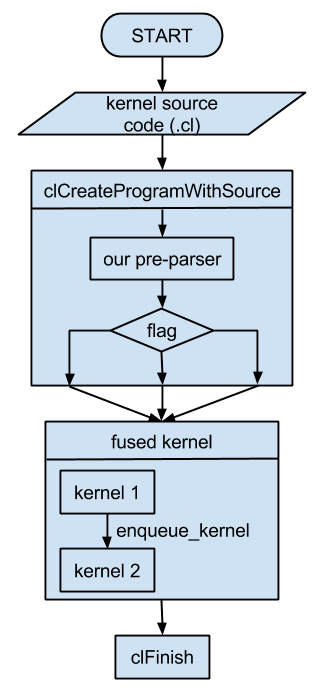
\includegraphics[width=5cm]{img/overview-approach.png}
\caption{Flowchart of approach}
\label{fig:my_label6}
\end{figure}

	If the last flag is specified, we will switch the enqueue command to the last line of the kernel. And then branch to the new kernel using block. This will let all work items within a work group wait for all work items to finish their previous kernel, and then branch to the new kernel by block.
	If the second flag is specified, we will switch the enqueue command to the last line with a barrier before it. But this will not let all work group wait for the others to finish the previous kernel, since synchronization between work groups cannot be done using OpenCL currently.
	If the first flag is specified, we will immediately branch to the new kernel by block. So the current kernel will be blocked and wait for the new kernel to finish. But the full functionality of the first flag should be enqueueing the new kernel, and then create a new thread for the new kernel. So the new kernel and the current kernel can be running at the same time. This will give the process better performance than our approach. But the first flag won’t be used when performing kernel fusion. The new kernel should have no dependency with the original kernel, since they should run at the same time.
	
\subsection{Comparison between two features}
\quad\ \ Besides Halide schedule “compute\_at” need to do redundant works, while our approach may not need to, one more difference is that our approach supports deciding which kernel to be fused at runtime. This can be used to perform dynamic kernel fusion while Halide schedule “compute\_at” can not. Halide schedule compute\_at need to decide which kernel to be fused at compile time, and Halide CodeGen will generate the corresponding OpenCL host and device source code.

\subsection{Different Approach: enqueue\_kernel}
\quad\ \ According to the original OpenCL 2.0 spec, there are some more built-in functions, host CL APIs, helper functions and data type definitions that need to be supported. Including host CL APIs clCreateCommandQueueWithProperties, built-in function get\_default\_queue. 
	clCreateCommandQueueWithProperties can be used to create a command queue with different properties supported. Since with different kernel enqueued, we may need command queue with different properties. The properties will be stored as a list. And the get\_default\_queue built-in function will be used to get the default device queue during the kernel (device queue is supposed to be the default command queue, in order to put the new enqueue kernel command into the default command queue.) 
	
	By using the host API clCreateCommandQueueWithProperties and the built-in function get\_default\_queue, we can put the kernel which we want to enqueue in the current kernel into the default command queue which we can obtain from get\_default\_queue and then enqueue it through the OpenCL command queue feature.
	
	But the difficulty here is, according to the OpenCL 2.0 spec, the enqueue\_kernel built-in function’s input argument is “block” which is defined by the Clang (a compiler front end for the C, C++, Objective-C and Objective-C++ programming languages.) It can be used like a function pointer, so we can not directly obtain the kernel name mapping to this block. But in POCL, we need to first create the whole program by clCreateProgramWithSource to create the binary. It will be compiled to .bc through LLVM (Low Level Virtual Machine), and then being compiled to .so. To enqueue a kernel, we need its kernel name to search for the code section in the .so file. The enqueue command in the command queue should contain the kernel name, which we currently do not have.
	
\subsection{Temporary storage allocation}
\quad\ \ To use enqueue\_kernel, we will need to allocate temporary storage. Since the output of the previous kernel will be the input of the next kernel, we need a temporary storage to store these data for the next kernel to read them. The storage type should be declared global, so all work items within all work groups can read it.

    We will need to allocate temporary storage at the host source code, and use allocated temporary storage instead of the original storing destination at the kernel source code.

\section{Experiments}
\quad\ \ This chapter contains three parts. The first part will show how much compile time our approach will increase. The second part will show the evaluations of image processing processes' total execution time comparison. The last part will show the evaluations of image processing processes' kernel execution time comparison, including doing kernel fusion by Halide schedule “compute\_at” and our “enqueue\_kernel" approach.

\subsection{compile time increase}
\quad\ \ We normalize compile time to OpenCL without pre-parser shown in figure~\ref{fig:my_label_ex_1}. The compile time includes time of OpenCL host API clCreateProgramWithSource. We can see that our pre-parser does not effect the compile time much.

\begin{figure}[hbtp]
\centering
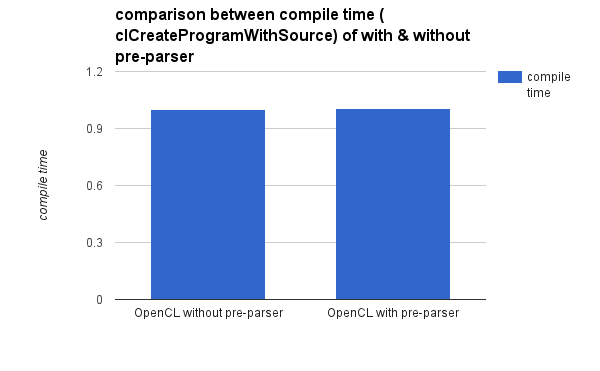
\includegraphics[width=7cm]{img/compile-time.png}
\caption{}
\label{fig:my_label_ex_1}
\end{figure}

\subsection{total execution time comparison}
\quad\ \ We normalize total execution time to OpenCL with kernel fusion shown in figure~\ref{fig:my_label_ex_2}. Since the benefit we can gain by doing kernel fusion will be a constant (OpenCL host APIs overhead), our speedup will decrease as the kernel execution time increase. The total execution time here includes whole OpenCL execution time except compile time (clCreateProgramWithSource.)
    
\begin{figure}[hbtp]
\centering
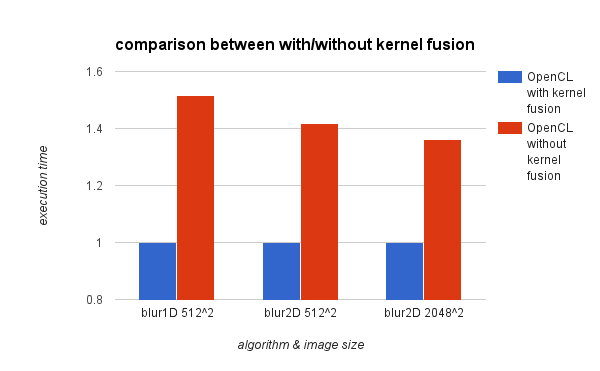
\includegraphics[width=7cm]{img/with-without-2ker.png}
\caption{total execution time comparison between OpenCL with \& without kernel fusion, fusing two kernels into one kernel}
\label{fig:my_label_ex_2}
\end{figure}

\subsection{kernel execution time comparison}
\quad\ \ We normalize kernel execution time to OpenCL without kernel fusion shown in figure~\ref{fig:my_label_ex_3}. The kernel execution time only includes the time of clEnqueueNDRangeKernel. We set a clWaitForEvents call to wait for the execution event to return and then get the execution time by clGetProfilingInfo. From this figure, we can see that our approach does not have big impact to the kernel execution time.
    
\begin{figure}[hbtp]
\centering
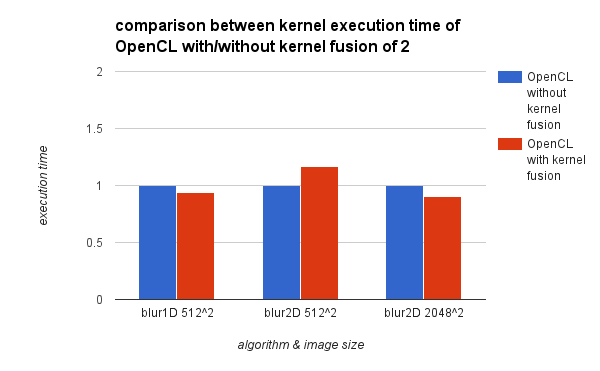
\includegraphics[width=7cm]{img/OpenCL-with-without-execute-2ker.png}
\caption{kernel execution time comparison between OpenCL with \& without kernel fusion, fusing two kernels into one kernel}
\label{fig:my_label_ex_3}
\end{figure}

    We normalize kernel execution time to Halide without kernel fusion shown in figure~\ref{fig:my_label_ex_4}. We can see that the execution time increases as the image kernel size increases or the image size increases.

\begin{figure}[hbtp]
\centering
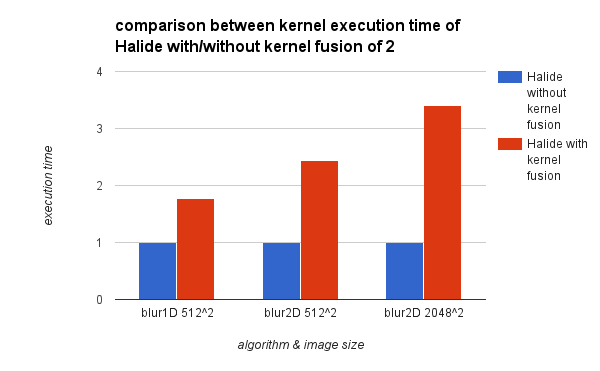
\includegraphics[width=7cm]{img/Halide-with-without-execute-2ker.png}
\caption{kernel execution time comparison between Halide with \& without kernel fusion, fusing two kernels into one kernel}
\label{fig:my_label_ex_4}
\end{figure}

    We normalize kernel execution time to Halide OpenCL CodeGen shown in figure~\ref{fig:my_label_ex_5}. We can see that the kernel execution time of Halide OpenCL CodeGen and our handwritten OpenCL source code are approximately equal. We believe that our handwritten OpenCL source code will do approximately equal operations to Halide OpenCL CodeGen.

\begin{figure}[hbtp]
\centering
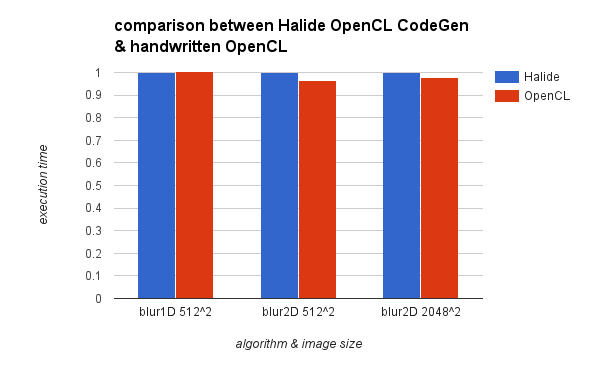
\includegraphics[width=7cm]{img/Halide-OpenCL-1ker-comp.png}
\caption{kernel execution time comparison between Halide OpenCL CodeGen \& handwritten OpenCL code, executing single kernel}
\label{fig:my_label_ex_5}
\end{figure}

    We normalize kernel execution time to our handwritten OpenCL source code shown in figure~\ref{fig:my_label_ex_6}. We can see the performances applying our approach are better than the ones applying Halide kernel fusion. These performance differences are due to the redundant works, which increase as the image kernel size increase or image size increase.

\begin{figure}[hbtp]
\centering
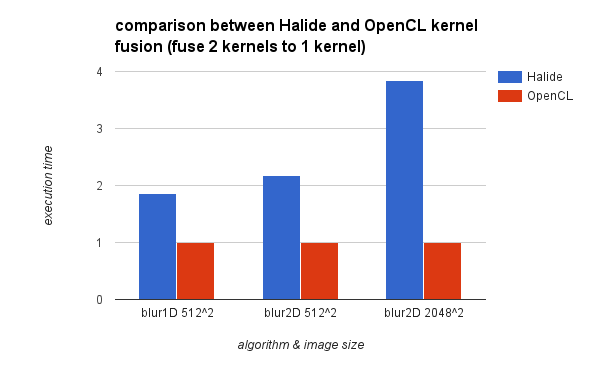
\includegraphics[width=7cm]{img/Halide-OpenCL-2ker-comp.png}
\caption{kernel execution time comparison between Halide \& OpenCL kernel fusion, fusing two kernels into one kernel}
\label{fig:my_label_ex_6}
\end{figure}

\section{Future Work}
\quad\ \ For the future work, we have three things to do. First, we should add our enqueue\_kernel approach to Halide OpenCL CodeGen and add automatic temporary storage allocation and using them in the kernel source code which we generated. This should improve the OpenCL performance of Halide.

    Second, we need to add temporary storage allocation into Halide OpenCL CodeGen, including OpenCL host source code and kernel source code. Since we need to do allocation at the host part, and change the usage and storing destination to our new allocated temporary storage at the kernel part.

    Last, we should implement full functionality of enqueue\_kernel with the first flag mentioned, CLK\_ENQUEUE\_FLAGS\_NO\_WAIT. This will offer us a new way to improve performance, because we can separate the works that have no dependency issues, and then enqueue a new kernel for these works. And we should also implement full functionality of CLK\_ENQUEUE\_FLAGS\_WAIT\_KERNEL, thus we can use enqueue\_kernel more flexibly and can make sure all work group finish the previous kernel.
    
\section{Conclusion}
\quad\ \ Fusing kernels into one big kernel can reduce OpenCL host APIs overhead. But as the tradeoff, we will need to do redundant works to compute the data needed. This may cause significant performance decreasing if the image kernel too big or the image size too huge. So we introduce another way to do kernel fusion without redundant works. But as the tradeoff, we will have barrier and temporary storge overheads. From the experiment result shown in chapter 5, we can believe that applying our approach to Halide's OpenCL CodeGen will increase the performance of kernel fusion.


\appendix
\section{Appendix Title}

This is the text of the appendix, if you need one.

\acks

Acknowledgments, if needed.

% We recommend abbrvnat bibliography style.

\nocite{*}
\bibliographystyle{abbrvnat}
\bibliography{thesis}

% The bibliography should be embedded for final submission.

%\begin{thebibliography}{}
%\softraggedright

%\bibliography{thesis}
%\bibitem[Smith et~al.(2009)Smith, Jones]{smith02}
%P. Q. Smith, and X. Y. Jones. ...reference text...


%\end{thebibliography}




\end{document}

%                       Revision History
%                       -------- -------
%  Date         Person  Ver.    Change
%  ----         ------  ----    ------

%  2013.06.29   TU      0.1--4  comments on permission/copyright notices

